\section{Εισαγωγή}
\subsection{\texorpdfstring{Γενικά για τα τσουνάμι}{}}
\paragraph{} Τα τσουνάμι (στα ιαπωνικά ((κύμα στο λιμάνι))) είναι κύματα που
δημιουργούνται από την απότομη μετατόπιση μεγάλων υδάτινων μαζών, συνήθως ως αποτέλεσμα
γεωλογικών φαινομένων (σεισμοί, εκρήξεις ηφαιστείων, κατολισθήσεις βράχων ή παγετώνων,
πτώση μετεωρίτη) σε παρα/υπο-θαλάσσιες τοποθεσίες). Λόγω του τρόπου δημιουργίας τους, τα
τσουνάμι είναι εντελώς διαφορετικά από τα συνηθισμέντα κύματα που δημιουργούνται από τον
άνεμο, οδεύοντας στον ανοιχτό, βαθύ ωκεανό με τεράστια ταχύτητα (750 \eng{km/h}) και μήκος
κύματος (50-400 \eng{km}), αλλά μικρό ύψος, που κυμαίνεται από μερικά \eng{cm} έως
\eng{1-2 m}. Προσεγγίζοντας πιο ρηχές περιοχές, το κύμα αλλάζει χαρακτηριστικά, καθώς η
ταχύτητα και το μήκος κύματος μειώνονται (κάτω από 80 \eng{km/h} και 20 \eng{km}
αντίστοιχα), ενώ το ύψος αυξάνεται. Ωστόσο, μόνο τα πολύ μεγάλα κύματα παρουσιάζουν
((σπάσιμο)) (\eng{wave breaking}), δηλαδή κατάρρευση της κορυφής τους, με αποτέλεσμα τα
τσουνάμι να μοιάζουν με μεγάλες και απότομες παλίρροιες που προσεγγίζουν ταχέως την
ακτή\footnote{Σ' αυτό οφείλεται και η συχνή αλλά εσφαλμένη αναφορά των κυμάτων αυτών ως
  παλιρροιακά κύματα.}. Λόγω της τεράστιας ενέργειας που μεταφέρουν (αυτή της μετατόπισης
ολόκληρης της υδάτινης στήλης που προκλήθηκε από το γενεσιουργό συμβάν) τα τσουνάμι είναι
καταστροφικά κατά την πρόσπτωσή τους στις ακτές. Με αυτόν τον τρόπο πήραν και το όνομά
τους, καθώς Ιάπωνες ψαράδες που έβγαιναν στα ανοιχτά δεν αντιλαμβάνονταν το τσουνάμι που
περνούσε κάτω από τα πλοία τους, αντίκριζαν όμως την ολική καταστροφή που είχε προκαλέσει
όταν γύριζαν στο λιμάνι. Τα πρόσφατα τσουνάμι στη νοτιοανατολική Ασία το 2004 και στην
Ιαπωνία το 2011 υπήρξαν δύο από τις μεγαλύτερες φυσικές καταστροφές στη σύγχρονη ιστορία,
με τεράστιο αριθμό θυμάτων και σοβαρές επιπτώσεις, βραχύχρονες (καταστροφή κτιρίων και
τοπικών υποδομών) και μακρόχρονες (καταστροφή και μεγάλη διαρροή ραδιενέργειας στον
πυρηνικό αντιδραστήρα της επαρχίας Φουκουσίμα στην Ιαπωνία). Σήμερα, περιοχές υψηλού
κίνδυνου διαθέτουν συστήματα προειδοποίησης τα οποία επεξεργαζόμενα γεωλογικά,
ωκεανογραφικά και σεισμολογικά δεδομένα σε πραγματικό χρόνο προειδοποιούν για επικείμενα
τσουνάμι.

\paragraph{} Εξαιτίας των σοβαρών τους επιπτώσεων, τα τσουνάμι έχουν αποτελέσει θέμα
εκτενούς μελέτης που αποσκοπεί στην κατανόηση, πρόβλεψη και πρόληψη ζημιών στο μέγιστο
δυνατό βαθμό. Η μελέτη επικεντρώνεται τόσο την ανάλυση δεδομένων σε παρελθόντα περιστατικά
\cite{Kanamori1972346, ABE19791561}, όσο και στην μελέτη-προσομοίωση του φαινομένου. Σε
αντίθεση με τις μεγάλης κλίμακας μελέτες (σε επίπεδο δεκάδων \eng{km}), οι οποίες αφορούν
τη γένεση/διάδοση των κυμάτων στον ανοιχτό ωκεανό και τα χαρακτηριστικά τους σε
μακροσκοπικό επίπεδο \cite{Shuto1991171, Titov23092005, Grilli2007414}, οι μικρής κλίμακας
προσομοιώσεις απαιτούν τον πλήρη συνυπολογισμό της ρευστομηχανικής συμπεριφοράς του
κύματος για την εξαγωγή σωστών αποτελεσμάτων, ο οποίος επιτυγχάνεται είτε με την
αριθμητική επίλυση διαφορικών εξισώσεων που περιγράφουν το κύμα, είτε με τη χρήση
σωματιδιακών μοντέλων \cite{goto1997iugg}.

\paragraph{} Υπάρχουν πολλές μέθοδοι προσομοίωσης ρευστών, καθεμία με πλεονεκτήματα και
μειονεκτήματα σε ένα πλήθος παραγόντων, όπως την ευστάθεια, την ακρίβεια, τον υπολογιστικό
φόρτο και τον χειρισμό οριακών συνθηκών και διαφορετικών φάσεων στο σύστημα
\cite{Tan2009723}. Οι κυριότερες παραδοσιακές μέθοδοι ανάλυσης/προσομοίωσης στηρίζονται
στην αριθμητική επίλυση ειδικών μορφών της εξίσωσης \eng{Navier-Stokes}
(\ref{eq:navier-stokes}) που προκύπτουν υπό παραδοχές και διαφορετικού βαθμού
απλοποιήσεις. Τέτοιες μορφές είναι οι εξισώσεις ρηχού νερού (\eng{SWE -- Shallow Water
  Equations} ή εξισώσεις \eng{Saint-Venant}), οι οποίες προκύπτουν υπό την παραδοχή οτι το
οριζόντιο χαρακτηριστικό μήκος της ροής είναι πολύ μεγαλύτερο από το βάθος του ρευστού
\cite{audusse2004fast, brodtkorb2012efficient}. Η προσέγγιση \eng{Boussinesq} βελτιώνει
την προηγούμενη ενσωματώνοντας και την συχνοτική διασπορά (\eng{frequency dispersion},
φαινόμενο κατά το οποίο κύματα με διαφορετικό μήκος κύματος ταξιδεύουν με διαφορετικές
ταχύτητες φάσης) \cite{watts2003landslide}, ενώ έχουν προταθεί και άλλες, πιο ακριβείς
μέθοδοι \cite{camassa1993integrable}. Απώτερος σκοπός της παρούσας εργασίας ήταν η κατα το
δυνατόν ακριβέστερη καταγραφή της μεταφοράς ορμής/ενέργειας από το νερό στην ακτογραμμή,
για την εκτίμηση των επιπτώσεων της πρόσκρουσης του τσουνάμι. Για το λόγο αυτό, επελέγη
σωματιδιακή μέθοδος προσομοίωσης, καθώς τέτοιες μέθοδοι εν\-δεί\-κνυ\-νται για
αλληλεπίδραση ρευστού με πολύπλοκες επιφάνειες (ελέυθερες και μη) παρέχοντας παράλληλα
άμεση πληροφορία σχετικά με αυτή, σε σχέση με αυτές που βασίζονται στην αριθμητική επίλυση
διαφορικών εξισώσεων. Οι δύο ευρύτερα χρησιμοποιουμενες σωματιδιακές μέθοδοι είναι η
\eng{Lattice Boltzmann Method (LBM)} και η \eng{Smoothed Particle Hydrodynamics (SPH)}.

\subsection{\texorpdfstring{\eng{Lattice Boltzmann Method}}{}}
\paragraph{} Η μέθοδος \eng{Lattice Boltzmann} \cite{chen1998329} βασίζεται στην
μεσοσκοπική θεώρηση του ρευστού, όπως αυτή περιγράφεται στην κινητική θεωρία από την
εξίσωση \eng{Boltzmann}:
\[
\frac{\partial f}{\partial t} +
\frac{\vec{p}}{m} \cdot \nabla f +
\vec{F} \cdot \frac{\partial f}{\partial \vec{p}} =
\left( \frac{\partial f}{\partial t} \right)_{\hspace{-2pt}\text{\eng{coll}}},
\]
όπου $f$
η συνάρτηση κατανομής των σωματιδίων του ρευστού στον εξαδιάστατο χώρο κατάστασης του
συστήματος (θέση και ορμή $\vec{p}$),
$m$
η μάζα των σωματιδίων, $\vec{F}$
το πεδίο εξωτερικών δυνάμεων που επιδρούν στα σωματίδια, ενώ το δεξί μέλος ισούται με τη
μεταβολή της $f$
λόγω συγκρούσεων μεταξύ των σωματιδίων. Κατά τη διάρκεια της προσομοίωσης, ο χώρος
κατάστασης του συστήματος και ο χρόνος διακριτοποιούνται και λαμβάνουν χώρα αλληλοδιάδοχα
βήματα συγκρούσης (\eng{collision}) και ροής (\eng{streaming}):
\begin{itemize}
\item[] \makebox[2cm]{Σύγκρουση:\hfill}
  $f_i(\vec{x},t+\delta_t) = f_i(\vec{x},t)+\frac{1}{\tau_f}(f_i^{\text{\eng{eq}}}-f_i)$
\item[] \makebox[2cm]{Ροή:\hfill}
  $f_i(\vec{x}+\vec{e}_i\delta_t, t+\delta_t)=f_i(\vec{x},t+\delta_t)$
\end{itemize}
Με δείκτη $i$ συμβολίζονται οι διακριτοποιημένες κατευθύνσεις της ορμής, με $\vec{e}_i$ τα
μοναδιαία διανύσματα κατά μήκος αυτών, με $\tau_f$ ο συντελεστής χαλάρωσης προς την
κατάσταση ισορροπίας $f_i^{eq}$ και με $\delta_t$ το χρονικό βήμα της προσομοίωσης.

\paragraph{} Η μέθοδος διαθέτει αρκετά πλεονεκτήματα τα οποία την καθιστούν ελκυστική σε
ορισμένες εφαρμογές. Λόγω της τοπικότητας και κανονικότητας της επεξεργασίας και κίνησης
των δεδομένων ταιριάζει ιδιαίτερα σε \eng{SIMD} αρχιτεκτονικές παράλληλης επεξεργασίας, οι
οποίες τα τελευταία χρόνια παρουσιάζουν τεράστια ανάπτυξη (π.χ. \eng{GPGPUs})
\cite{Bailey2009550, Kuznik20102380}. Επίσης διακρίνεται για την ευκολία με την οποία
χειρίζεται ροές με πολλές φάσεις που πιθανόν αλληλεπιδρούν με συγκεκριμένο τρόπο και σε
περίπλοκη γεωμετρία (όπως πορώδη μέσα). Αν και έχει γίνει σημαντική δουλειά στη χρήση της
μεθόδου για προσομοίωση φαινομένων που άπτονται της παρούσας εργασίας τόσο σε θεωρητικό
\cite{Zhou20023527, Zhou2004lattice} όσο και σε τεχνικό επίπεδο \cite{Krafczyk2007,
  Janssen2012efficient}, η \eng{LBM} διαθέτοντας μεγάλο θεωρητικό υπόβαθρο αποτελεί
αντικείμενο ενεργούς έρευνας για διεύρυνση και βελτίωση της εφαρμογής της προς κάθε
κατεύθυνση.

\subsection{\texorpdfstring{\eng{Smoothed Particle Hydrodynamics}}{}}
\paragraph{} Η \eng{SPH} είναι μια Λαγκρανζιανή\footnote{Σε αντίθεση με την Οϊλεριανή
  (\eng{Eulerian}) θεώρηση, όπου η ροή περιγράφεται ως συνάρτηση της θέσης και του χρόνου,
  στις Λαγκρανζιανές (\eng{Lagrangian}) μεθόδους τμήματα του ρευστού (\eng{fluid parcels})
  αποτελούν τα σημεία αναφοράς.} μέθοδος προσομοίωσης ρευστών που εισήχθη τη δεκαετία του
1970 για εφαρμογές στην αστροφυσική \cite{gingold1977375, lucy19771013} και έκτοτε έχει
βρει ευρύτατη εφαρμογή σε πολλά πεδία, όπως τη βαλλιστική, αεροδυναμική, ναυπηγική και
γραφικά \cite{monaghan20051703}. Θεμέλιο της μεθόδου αποτελεί η αντικατάσταση του ρευστού
από ένα σύνολο σωματιδίων, τα οποία φέρουν ιδιότητες του ρευστού και αποτελούν σημεία
παρεμβολής για τον υπολογισμό αυτών σε άλλα σημεία του χώρου, λόγω του οποίου διαθέτει
αρκετά πλεονεκτήματα:
\begin{itemize}
\item Εγγενής διατήρηση πολλών μεγεθών στο σύστημα λόγω της σωματιδιακής του φύσης, όπως
  μάζα, ορμή και ενέργεια.
\item Ακριβής, ισότροπος και αμετάβλητος σε κάθε αδρανειακό σύστημα αναφοράς
  (\eng{Galilean invariant}) χειρισμός της καθαρής μεταφοράς (\eng{pure advection})
\item Δυνατότητα προσαρμογής της αναλυτικότητας (\eng{resolution}) και κατά συνέπεια του
  υπολογιστικού φόρτου δυναμικά συναρτήσει της θέσης, χρόνου ή άλλων παραγόντων.
\item Εύκολος χειρισμός ορίων και ειδικών αλληλεπιδράσεων σε εφαρμογές με πολλές
  φάσεις/υλικά, μέσω των σωματιδιακών αλληλεπιδράσεων.
\end{itemize}

\subsubsection{Θεωρητική θεμελίωση}
\paragraph{} Έστω η ταυτότητα
\begin{equation}
  f(\vec{r}) = \int_Vf(\vec{x}) \delta(\vec{r} - \vec{x}) d\vec{x},
\end{equation}
όπου $f(\vec{r})$
μια συνάρτηση με πεδίο ορισμού το $V$, $\delta(\vec{r})$ η δέλτα του \eng{Dirac} και
$\vec{x} \in V$. Η συνάρτηση δέλτα μπορεί να θεωρηθεί η οριακή περίπτωση ενός πυρήνα
εξομάλυνσης $W(\vec{r}, h)$ με τις εξής ιδιότητες
\begin{equation}
  \label{eq:kernel-properties}
  \lim_{h\to0}W(\vec{r}, h) = \delta(\vec{r})\ \ \
  \text{και}\ \ \
  \int_VW(\vec{r}, h) d\vec{x} = 1
\end{equation}
Τότε, για μικρές τιμές του $h$ ισχύει
\begin{equation}
  \label{eq:c-approx}
  f(\vec{r}) \approx \int_V f(\vec{x}) W(\vec{r}-\vec{x}, h) d\vec{x}
\end{equation}
Αφού διακριτοποιήσουμε το πεδίο $f$
σε σωματίδια πυκνότητας $\rho_i$
και μάζας $m_i$
μπορούμε να πολλαπλασιάσουμε και να διαιρέσουμε με $\rho$
το δεξί μέλος της σχέσης \ref{eq:c-approx}, το οποίο μετατρέπεται πλέον σε διακριτό άθροισμα.
Παρατηρώντας ότι $\rho*d\vec{x} = m$,
καταλήγουμε στην ακόλουθη σχέση που αποτελεί τη βάση προσέγγισης οποιουδήποτε μεγέθους $A$
σύμφωνα με την \eng{SPH}
\begin{equation}
  \label{eq:d-approx}
  A(\vec{r}) \approx \sum_i \frac{m_i}{\rho_i} A(\vec{r}_i) W(\vec{r}-\vec{x}_i, h)
\end{equation}
Σύμφωνα με αυτή, η τιμή της $A$
σε μια θέση του χώρου $\vec{r}$
μπορεί να υπολογιστεί προσεγγιστικά απο το σταθμισμένο άθροισμα των τιμών της στα
γειτονικά σωματίδια $i$.
Η συνεισφορά κάθε σωματιδίου καθορίζεται τόσο από το λόγο της μάζας του προς την τοπική
πυκνότητα $m_i/\rho_i$, όσο και από την απόστασή του από το σημείο υπολογισμού της $A$
μέσω του πυρήνα $W(\vec{r}-\vec{x}_i, h)$.

\subsubsection{Διανυσματικοί τελεστές σε διακριτοποιημένα πεδία}
\label{sssec:vector-calc}
\paragraph{} Δεδομένου ότι $\nabla \equiv \partial/\partial\vec{r}$,
από τη σχέση \ref{eq:d-approx} για τη βάθμωση του μεγέθους $A$ προκύπτει
\begin{equation}
  \label{eq:d-grad}
  \nabla A(\vec{r}) \approx \sum_i \frac{m_i}{\rho_i} A(\vec{r}_i) \nabla W(\vec{r} - \vec{x}_i, h)
\end{equation}
Αντίστοιχα, για την απόκλιση και το στροβιλισμό του διανυσματικού μέγεθους $\vec{A}$
\begin{equation}
  \label{eq:d-div}
  \nabla \cdot \vec{A}(\vec{r}) \approx \sum_i \frac{m_i}{\rho_i} \vec{A}(\vec{r}_i)
  \cdot \nabla W(\vec{r} - \vec{x}_i, h)
\end{equation}
\begin{equation}
  \label{eq:d-curl}
  \nabla \times \vec{A}(\vec{r}) \approx \sum_i \frac{m_i}{\rho_i} \vec{A}(\vec{r}_i)
  \times \nabla W(\vec{r} - \vec{x}_i, h)
\end{equation}
Αξίζει να σημειωθεί η εξάρτηση της προσέγγισης αποκλειστικά από τις τιμές της συνάρτησης
$A(\vec{r}_i)$/$\vec{A}(\vec{r}_i)$
και της βάθμωσης του πυρήνα εξομάλυνσης $\nabla W$,
χαρακτηριστικό ιδιαίτερα χρήσιμο υπολογιστικά, καθώς η τελευταία μπορεί να
προϋπολογιστεί.

\paragraph{} Οι παραπάνω σχέσεις μπορούν να τροποποιηθούν για την ικανοποίηση ειδικών
συνθηκών της εκάστοτε εφαρμογής. Στην παρούσα περίπτωση απαιτείται η διατήρηση της ορμής
στο ρευστό, η οποία μεταφράζεται στην εξασφάλιση αντισυμμετρικών δυνάμεων (δράσης -
αντίδρασης) μεταξύ των σωματιδίων του ρευστού. Η εξίσωση \eng{Navier-Stokes}
\begin{equation}
  \label{eq:navier-stokes}
  \rho \left( \frac{\partial \vec{v}}{\partial t} + \vec{v} \cdot \nabla \vec{v} \right) =
  \rho \vec{g} - \nabla P + \mu \nabla^2 \vec{v},
\end{equation}
όπου $\rho$
η πυκνότητα, $\vec{v}$
η ταχύτητα, $P$
η πίεση, $\vec{g}$
η πυκνότητα εξωτερικών δυνάμεων και $\mu$
το δυναμικό ιξώδες του ρευστού, είναι η έκφραση του δεύτερου νόμου του \eng{Newton} για
ρευστά. Σύμφωνα με αυτή, οι εσωτερικές δυνάμεις του ρευστού οφείλονται στη βάθμωση του
πεδίου πίεσης και το γινόμενο του δυναμικού ιξώδους με τη λαπλασιανή του πεδίου
ταχύτητας. Μπορούμε να καταλήξουμε σε διαφορετικό εκτιμητή για τη βάθμωση της πίεσης
ξεκινώντας από την ταυτότητα
\begin{equation*}
  \label{eq:grad-identity}
  \nabla \left( \frac{P}{\rho} \right) =
  \frac{\nabla P}{\rho}-
  \frac{P}{\rho^2} \nabla \rho
  \hspace{10pt} \Leftrightarrow \hspace{10pt}
  \nabla P = \rho \left[ \frac{P}{\rho^2} \nabla \rho + \nabla \left( \frac{P}{\rho}
    \right) \right]
\end{equation*}
Αντικαθιστώντας στο δεξί μέλος τις βαθμώσεις με τους εκτιμητές τους κατά \eng{SPH}
\begin{align}
  \label{eq:grad-est}
  \nabla P &\approx \rho \left[ \frac{P}{\rho^2} \sum_i \frac{m_i}{\rho_i} \rho \nabla
             W(\vec{r}-\vec{r}_i, h)
             +
             \sum_i \frac{m_i}{\rho_i} \frac{P_i}{\rho_i} \nabla W(\vec{r}-\vec{r}_i, h)
             \right] \nonumber \\
           &\approx\rho \sum_i m_i \left(\frac{P}{\rho^2} + \frac{P_i}{\rho_i} \right)
             \nabla W(\vec{r}-\vec{r}_i, h)
\end{align}
προκύπτει η σχέση που χρησιμοποιείται ευρύτατα για την εκτίμηση της βάθμωσης της πίεσης
και ικανοποιεί παράλληλα τη συνθήκη αντισυμμετρικότητας για τη διατήρηση της ορμής και
στροφορμής. Παρόμοια, για τη λαπλασιανή του πεδίου ταχύτητας χρησιμοποιείται συνήθως η
προσέγγιση
\begin{equation}
  \label{eq:lapl-est}
  \nabla^2\vec{v} \approx \sum_i \frac{m_i}{\rho_i} (\vec{v}_i - \vec{v}) \nabla^2
  W(\vec{r}-\vec{r}_i, h)
\end{equation}
η οποία διαθέτει την επιθυμητή για την προσομοίωση των δυνάμεων ιξώδους ιδιότητα του
μηδενισμού σε κατάσταση ομοιόμορφης μεταφορικής κίνησης του ρευστού (ίση ταχύτητα στο
εύρος του πυρήνα εξομάλυνσης).

\subsubsection{Καταστατική εξίσωση}
\paragraph{} Για τον υπολογισμό της βάθμωσης της πίεσης είναι απαραίτητος ο υπολογισμός
των τιμών της στα σημεία δειγματοληψίας (σωματίδια). Αυτός γίνεται με τη βοήθεια μιας
καταστατικής εξίσωσης, η οποία συσχετίζει την πυκνότητα με την πίεση του ρευστού. Επομένως
για να εκτιμηθεί η πίεση σε κάποιο σημείο πρέπει πρώτα να εκτιμηθεί η πυκνότητα στο σημείο
αυτό από τη σχέση \ref{eq:d-approx}:
\begin{equation}
  \label{eq:dens-est}
  \rho(\vec{r}) \approx \sum_i m_i W(\vec{r}-\vec{x}_i, h)
\end{equation}
Οι δύο ευρύτερα χρησιμοποιούμενες καταστατικές εξισώσεις είναι αυτή των ιδανικών αερίων
\cite{muller2003particle, desbrun1996smoothed}
\begin{equation}
  \label{eq:ideal_state}
  P = k(\rho - \rho_0),
\end{equation}
που συσχετίζει την πίεση με την απόκλιση από την πυκνότητα αναφοράς $\rho_0$
με μια σταθερά αναλογίας $k$,
καθώς και η εξίσωση \eng{Tait} \cite{becker2007weakly, monaghan20051703}
\begin{equation}
  \label{eq:tait_state}
  P = B \left( \left( \frac{\rho}{\rho_0} \right)^\gamma - 1 \right),
\end{equation}
όπου $\gamma=7$
αδιάστατη σταθερά και $B$
σταθερά αναλογίας που ρυθμίζει την ανοχή στις διακυμάνσεις της πυκνότητας. Η τιμή της $B$
καθορίζεται βάσει της αναλογίας
\begin{equation}
  \label{eq:compressibility_scale}
  \frac{|\Delta\rho|}{\rho_0} \sim \frac{\|\vec{v}_f\|^2}{c_s^2},
\end{equation}
όπου $\Delta\rho = \rho - \rho_0$,
$\vec{v}_f$
η ταχύτητα της ροής και $c_s$
η ταχύτητα του ήχου στο ρευστό. Εάν θέσουμε $\eta = |\Delta\rho|/\rho_0$,
τότε ισοδύναμα ισχύει $c_s \sim \vec{v}_f / \sqrt{\eta}$.
Μπορεί να τεθεί άνω όριο για το $\eta$
(λ.χ. $\eta = 0.01$
για διακυμάνσεις πυκνότητας της τάξης του $1\%$),
το οποίο επιβάλλεται στην προσομοίωση θέτοντας $B = \rho_0 c_s^2 / \gamma$.
Ωστόσο, για λόγους ευστάθειας, η χρήση της εξίσωσης \eng{Tait} απαιτεί πολύ μικρό χρονικό
βήμα, λόγω της παρουσίας του $c_s^2$ στο συντελεστή αναλογίας $B$.

\subsubsection{Πυρήνες εξομάλυνσης}
\paragraph{} Από τα παραπάνω γίνεται σαφές οτι η επιλογή του πυρήνα εξομάλυνσης είναι
σημαντική, καθώς από αυτήν εξαρτάται άμεσα η ακρίβεια των προσεγγίσεων στο
διακριτοποιημένο ρευστό. Ο πυρήνας εξομάλυνσης θα πρέπει να ικανοποιεί τις σχέσεις
\ref{eq:kernel-properties}, να είναι συνεχής και παραγωγίσιμος (για τον υπολογισμό των
προσεγγίσεων διαφορικών τελεστών) καθώς και σφαιρικά συμμετρικός, ώστε οι τιμές του να
εξαρτώνται αποκλειστικά από την απόσταση από το κέντρο του $r = \|\vec{r}-\vec{r}_i\|$
και την ακτίνα εξομάλυνσης $h$.
Συνήθως χρησιμοποιούνται διαφορετικοί πυρήνες για κάθε προσεγγιζόμενο μέγεθος, αναλόγως
των ειδικών συνθηκών που απαιτούνται για την προσομοίωση της συμπεριφοράς που αυτό
προκαλεί \cite{muller2003particle}

\begin{figure}[h]
  \centering
  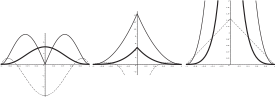
\includegraphics[width=\textwidth]{figures/smoothing-kernels.pdf}
  \caption[Πυρήνες εξομάλυνσης] {Οι τρεις πυρήνες εξομάλυνσης $W_{\text{\eng{poly6}}}$
    $W_{\text{\eng{spiky}}}$
    και $W_{\text{\eng{viscosity}}}$
    (από δεξιά προς τα αριστερά). Με τονισμένη γραμμή απεικονίζεται ο πυρήνας, με λεπτή η
    βάθμωσή του (στην κατεύθυνση προς την αρχή των αξόνων) και με διακεκομένη η λαπλασιανή
    του, για ακτίνα εξομάλυνσης $h=1$.
    (από \eng{M{\"u}ller et al, 2003}) \cite{muller2003particle}}
  \label{fig:smoothing-kernels}
\end{figure}

\paragraph{} Στο σχήμα \ref{fig:smoothing-kernels} φαίνονται οι τρεις πυρήνες
$W_{\text{\eng{poly6}}}$
$W_{\text{\eng{spiky}}}$
και $W_{\text{\eng{viscosity}}}$
που χρησιμοποιούνται πρακτικά για τον υπολογισμό της πυκνότητας, της βάθμωσης της πίεσης
και της λαπλασιανής του πεδίου ταχύτητας αντίστοιχα. Είναι σημαντικό για την ευστάθεια της
προσομοίωσης, αλλά και λογικό από φυσικής εποπτείας οι πυρήνες και οι παράγωγοι τους να
τείνουν στο μηδέν στα όρια της ακτίνας εξομάλυνσης. Για τον υπολογισμό της πυκνότητας
χρησιμοποιείται ο πυρήνας
\begin{equation}
  \label{eq:poly6}
  W_{\text{\eng{poly6}}}(r, h) = \frac{315}{64 \pi h^9}
  \begin{cases}
    (h^2 - r^2)^3 & 0 \leq r \leq h\\
    0 & \text{διαφορετικά}
  \end{cases}
\end{equation}
ο οποίος είναι τυπικός κωδωνοειδής πληρώντας τα χαρακτηριστικά που αναφέρθηκαν
προηγουμένως. Παρ' όλ' αυτά δε χρησιμοποιείται για την προσέγγιση της βάθμωσης της πίεσης,
καθότι η μηδενική παράγωγος στο κέντρο οδηγεί σε συσσωμάτωση (\eng{clustering}) των
σωματιδίων λόγω απουσίας απωστικών δυνάμεων μεταξύ τους. Για το λόγο αυτό, έχει προταθεί
\cite{desbrun1996smoothed} ο πυρήνας
\begin{equation}
  \label{eq:spiky}
  W_{\text{\eng{spiky}}}(r, h) = \frac{15}{\pi h^6}
  \begin{cases}
    (h - r)^3 & 0 \leq r \leq h\\
    0 & \text{διαφορετικά}
  \end{cases}
\end{equation}
\begin{equation}
  \label{eq:spiky-gradient}
  \nabla W_{\text{\eng{spiky}}}(r, h) = \frac{-45}{\pi h^6} (h-r)^2
\end{equation}
για τον υπολογισμό των δυνάμεων οφειλομένων στη βάθμωση της πίεσης. Ωστόσο οι δυνάμεις
ιξώδους είναι ανάλογες της λαπλασιανής του πυρήνα, με αποτέλεσμα οι παραπάνω πυρήνες να
είναι ακατάλληλοι για την προσέγγισή τους. Δεδομένου οτι οι δυνάμεις αυτές οφείλονται στην
εσωτερική τριβή του ρευστού, έχουν πάντα αποσβεστικά αποτελέσματα αμβλύνοντας τις τοπικές
διαφορές στην ταχύτητά του. Αντίθετα, οι λαπλασιανές των παραπάνω πυρήνων αλλάζουν αλλάζει
πρόσημο παίρνοντας αρνητικές τιμές. Έτσι υιοθετείται ο πυρήνας
\begin{equation}
  \label{eq:viscosity}
  W_{\text{\eng{viscosity}}}(r, h) = \frac{15}{2 \pi h^3}
  \begin{cases}
    - \frac{r^3}{2h^3} + \frac{r^2}{h^2} + \frac{h}{2r} - 1 & 0 \leq r \leq h\\
    0 & \text{διαφορετικά},
  \end{cases}\\
\end{equation}
\begin{equation}
  \label{eq:viscosity-laplacian}
  \nabla^2 W_{\text{\eng{viscosity}}}(r, h) = \frac{45}{\pi h^6} (h-r)
\end{equation}
ο οποίος έχει παντού θετική λαπλασιανή, της οποίας η γραμμικότητα συμβάλλει περαιτέρω στην
ευστάθεια της προσομοίωσης.

\subsubsection{Ολοκλήρωση και χρονικό βήμα}
\paragraph{} Εκτός της επιλογής του πυρήνα, καθοριστική για την ακρίβεια και ευστάθεια της
προσομοίωσης είναι η επιλογη του χρονικού βήματος και της μεθόδου ολοκλήρωσης στο
χρόνο. Το χρονικό βήμα υπολογίζεται συνήθως με βάση το κριτήριο \eng{CFL
  (Courant-Friedrichs-Lewy)} το οποίο στην απλούστερη μορφή του δίνεται από τη σχέση
\begin{equation}
  \label{eq:cfl}
  \delta t_{\text{\eng{CFL}}} = C \frac {\delta x}{v},
\end{equation}
όπου $C$
ο αδιάστατος αριθμός \eng{Courant} (συνήθως $0 < C \leq 1$),
$\delta x$
είναι κάποιο χαρακτηριστικό μήκος και $v$
μια σχετική με αυτό χαρακτηριστική ταχύτητα. Στην περίπτωση της \eng{SPH} μπορεί να
χρησιμοποιηθεί η ακτίνα εξομάλυνσης $h$
ή η ακτίνα των σωματιδίων σαν $\delta x$,
ενώ για την $v$
είτε η ταχύτητα του ήχου στο ρευστο, είτε η ταχύτητα των σωματιδίων για τη μέγιστη ανεκτή
μεταβολή πυκνότητας κατά τη διάρκεια ενός χρονικού βήματος, είτε η μέγιστη ταχύτητα των
σωματιδίων (αν μπορεί αυτή εκ των προτέρων να εκτιμηθεί με αξιοπιστία και δεν οδηγεί σε μη
αποδεκτές μεταβολές πυκνότητας). Μεταβλητό χρονικό βήμα μπορεί να χρησιμοποιηθεί υπό
προϋποθέσεις εξαρτώμενες και από την μέθοδο ολοκλήρωσης, με την προσαρμογή να λαμβάνει
χώρα σε κάθε βήμα της προσομοίωση με βάση το κριτήριο \eng{CFL} \cite{gomez2010state}.

\paragraph{} Για την αριθμητική ολοκλήρωση στο χρόνο χρησιμοποιούνται πολλές μέθοδοι,
μεταξύ των οποίων η \eng{predictor-corrector} και η \eng{Runge-Kutta-Fehlberg}. Ίσως η
ευρύτερα διαδεδομένη είναι η οικογένεια των \eng{St{\"o}rmer-Verlet} και \eng{Leapfrog},
οι οποίες είναι μέθοδοι δεύτερης τάξης με χαμηλές υπολογιστικές απαιτήσεις και καλή
αριθμητική ευστάθεια. Η μέθοδος \eng{Leapfrog} οφείλει το όνομά της στον αλληλοδιάδοχο
υπολογισμό της θέσης και της ταχύτας ανα μισό χρονικό βήμα
\begin{align}
  \begin{split}
    \label{eq:leapfrog}
    \vec{r}_{i+1} &= \vec{r}_i + \vec{v}_{i-1/2} \delta t \\
    \vec{v}_{i+1/2} &= \vec{v}_{i-1/2} + \vec{a}_i \delta t
  \end{split}
\end{align}
ή ισοδύναμα, σε ακέραια χρονικά βήματα
\begin{align}
  \begin{split}
    \label{eq:leapfrog}
    \vec{r}_{i+1} &= \vec{r}_i + \left( \vec{v}_i + \vec{a}_i \frac{\delta t}{2} \right) \delta t \\
    \vec{v}_{i+1} &= \vec{v}_i + \frac{\vec{a}_i + \vec{a}_{i+1}}{2} \delta t
  \end{split}
\end{align}
Λόγω της εξάρτησης των δυνάμεων (λ.χ. ιξώδους) και από την ταχύτητα στην \eng{SPH} μπορούν
να χρησιμοποιηθούν διάφορες τεχνικές εκτίμησης για τιμές στο μέλλον, όπως την επιτάχυνση
$\vec{a}_{i+1}$
\cite{rawiraswattana2012dynamics}.  Αυτές προσφέρουν παράλληλα τη δυνατότητα χρήσης
μεταβλητού χρονικού βήματος \cite{springel2001gadget}, η οποία δεν υπάρχει στην απλή
\eng{Leapfrog} μέθοδο, λόγω της εγγενούς συμμετρίας της \cite{skeel1993variable}.

%%% Local Variables:
%%% mode: latex
%%% TeX-master: "report"
%%% End:
